\documentclass[11pt]{article}
\usepackage[margin=1in]{geometry}
\usepackage{fontspec}
\usepackage{booktabs}
\usepackage{longtable}
\usepackage{array}
\usepackage{float}
\usepackage{graphicx}
\usepackage{adjustbox}
\usepackage[font=small,labelfont=bf]{caption}
\usepackage{natbib}
\usepackage{xurl}
\usepackage[hidelinks]{hyperref}
\usepackage{setspace}
\setstretch{1.15}
\setcitestyle{round,semicolon,aysep={},yysep={;}}
\graphicspath{{../figs/}}
% Generated by scripts/04_tables.R; do not edit.
\newcommand{\nStates}{3}
\newcommand{\nElections}{76}
\newcommand{\nElectionsPa}{30}
\newcommand{\nPersonElections}{550,331,623}
\newcommand{\nBirthday}{1,507,202}
\newcommand{\nRegistrantsFl}{15,378,113}
\newcommand{\window}{30}
\newcommand{\weekPooled}{0.35}
\newcommand{\weekPooledSe}{0.02}
\newcommand{\dayPooled}{0.53}
\newcommand{\dayPooledSe}{0.04}
\newcommand{\dayPooledRate}{40.4\%}
\newcommand{\dayPooledRelative}{1.3\%}
\newcommand{\birthdayPooled}{0.13}
\newcommand{\birthdayPooledSe}{0.05}
\newcommand{\birthdayPooledLo}{0.03}
\newcommand{\birthdayPooledHi}{0.22}
\newcommand{\dayFl}{0.45}
\newcommand{\dayOh}{0.54}
\newcommand{\dayPa}{0.61}
\newcommand{\birthdayFl}{0.05}
\newcommand{\birthdayOh}{0.30}
\newcommand{\birthdayPa}{0.08}
\newcommand{\pollsDayFl}{0.65}
\newcommand{\pollsDayPa}{0.71}
\newcommand{\pollsBirthdayFl}{0.39}
\newcommand{\earlyBirthdayFl}{0.28}
\newcommand{\mailBirthdayFl}{0.16}
\newcommand{\mailBirthdayPa}{0.19}
\newcommand{\replicationDay}{0.56}
\newcommand{\replicationDaySe}{0.05}
\newcommand{\discoveryDay}{0.48}
\newcommand{\settledDay}{0.58}
\newcommand{\allDay}{0.58}
\newcommand{\twowaySe}{0.05}
\newcommand{\farSd}{0.07}
\newcommand{\generalDay}{0.81}
\newcommand{\primaryDay}{0.45}
\newcommand{\placeboFrom}{8}
\newcommand{\registrationRatio}{4.8}
\newcommand{\threeDaysPooled}{0.43}
\newcommand{\threeDaysPooledSe}{0.03}
\newcommand{\twoWeeksPooled}{0.24}
\newcommand{\twoWeeksPooledSe}{0.02}

\newcommand{\TableStyle}{\normalsize\setlength{\tabcolsep}{6pt}\renewcommand{\arraystretch}{1}}


\title{Birthday Voter: How Birthdays Near Election Day Change Whether and How People Vote}
\author{Jake Leland \and Gaurav Sood}
\date{}

\begin{document}
\maketitle

\begin{abstract}
\noindent A birthday in the days before Election Day lowers turnout, and a birthday on Election Day changes it little. We use voter files from Florida, Ohio, and Pennsylvania covering \nElections{} statewide elections and \nPersonElections{} registrant-elections. Election dates move from year to year, so the same birth date falls on or near Election Day in some years and not others, and we compare people born on the same date across those years. A birthday the day before Election Day lowers turnout by \dayPooled{} percentage points (SE \dayPooledSe{}), about \dayPooledRelative{} of the turnout rate, and the estimate is similar in each state. An Election Day birthday raises turnout by \birthdayPooled{} points (95\% CI \birthdayPooledLo{} to \birthdayPooledHi{}), mostly in Ohio. The loss falls on voting in person. Where the files record how people voted, voting early or by mail rises around the birthday. We first saw the pattern in Florida's 2006--2016 elections, and it recurs in every sample not used to find it. Birthdays look less like an occasion for civic duty than like a claim on time that people plan around when the clash is exact but not when it is near.
\end{abstract}

\section{Introduction}

People are less likely to vote when their birthday falls in the days just before Election Day. Using voter files from three states, we find that a birthday the day before an election lowers turnout by about half a percentage point. A birthday on Election Day itself does not: people who would have voted at the polls that day vote early or by mail instead.

The pattern bears on why people vote. Few would vote if they voted only to change outcomes, because one vote almost never decides an election (\citealp{downs1957economic, mclean1994condorcet}; but see \citealp{edlin2007voting}). One explanation is that voting brings expressive benefits, among them the satisfaction of doing one's duty \citep{riker1968theory, fiorina1976voting, kan2001expressive}. Another is that voting costs little, so that small changes in its cost move turnout \citep{verba1993citizen}.

Birthdays separate these accounts. If people treat voting as a duty and like doing dutiful things on a day that feels significant, an Election Day birthday should raise turnout. If people take their birthday off work, voting should get cheaper, the logic behind proposals to make Election Day a holiday \citep{farber2009democracy}, and turnout should again rise. If a birthday competes for time, with a dinner, a trip, or a day spent elsewhere, it should lower turnout or move votes to other days. The evidence fits the last account.

\section{Data}

Table~\ref{tab:data} describes the data. For each state we have a voter file listing everyone registered when it was drawn, with their date of birth and registration date, and a history of their participation in past elections. The data are public records, distributed through the Harvard Dataverse; our replication materials contain counts by election and exact date of birth, with no names or identifiers.

\begin{table}[htbp]
\centering\TableStyle
\caption{Data. Elections are statewide general elections and primaries; registrants are those with a date of birth in the state's largest extract; person-elections are registrant-elections in the analysis sample; turnout is the share of them who voted.}
\label{tab:data}
\begin{adjustbox}{max width=\textwidth}
\begin{tabular}{lrrrrrl}
\toprule
State & Elections & Registrants & Person-elections & Birthday on E-Day & Turnout & Method recorded \\
\midrule
Florida & 20 (2006--2020) & 15,378,113 & 215,465,585 & 603,601 & 40.6\% & polls, early, mail \\
Ohio & 26 (2000--2016) & 7,891,442 & 135,241,890 & 365,341 & 49.9\% & -- \\
Pennsylvania & 30 (2009--2024) & 8,823,823 & 199,624,148 & 538,260 & 34.8\% & polls, mail \\
\bottomrule
\end{tabular}

\end{adjustbox}
\end{table}

\emph{Florida.} The February 2017 and June 2022 extracts of the Florida voter file record, for every election, whether a registrant voted at the polls on Election Day, voted early in person, voted by mail, or cast a ballot that was not counted. We take each election from the earliest extract filed after it, so a person on both lists contributes each election once. We use general elections, primaries, and presidential preference primaries from 2006 to 2020.

\emph{Ohio.} The 2016 statewide voter file (with history through May 2017) has a column for each election since 2000; an entry means the person voted, and the file does not say how. We use every November general election, including the odd-year elections in which Ohio votes on statewide issues, and the spring primaries of even years.

\emph{Pennsylvania.} The August 2024 Full Voter Export records each registrant's last 40 elections and how they voted: at the polls, absentee, by mail (from 2020), or provisionally. Pennsylvania has no early in-person voting. We use the \nElectionsPa{} elections that every county's record covers, November 2009 to April 2024.

Two features of the files matter for the design. First, each file lists only people registered when it was drawn, so turnout differs from official figures (Appendix Table~\ref{tab:elections}). It runs above them in older general elections, because people later removed from the rolls voted less, and below them in Florida's presidential preference primaries, whose denominators here include registrants not eligible to vote in a party's primary. These differences affect turnout levels, which the design absorbs, not the comparison of birthdays. Second, Ohio and Pennsylvania record a person's latest registration date, so we count someone as eligible for an election if that date clears the registration deadline or if they had voted in an earlier election.

\section{Research Design}

The unit is a registrant in an election, and the outcome is whether they voted. The quantity of interest is how turnout changes with the number of days between Election Day and the person's birthday that year, which we write $d$: $d = 0$ when Election Day is the birthday, $d = -1$ when the birthday was the day before.

People born at different times of year differ in many ways, so comparing people with $d = 0$ to everyone else would confound the birthday with the season of birth. Instead we compare people born on the same calendar date, in the same state and type of election, across elections in which that date fell at different distances from Election Day. The comparison works because election dates move. General elections fall between November 2 and 8; Pennsylvania's primaries have fallen anywhere from April 23 to June 2; and Ohio's primaries move between March and May. A person born on November 4 had a birthday on Election Day in some general elections and a few days before or after it in others. Birth dates close to Election Day never fall far from it within one type of election, so their estimates come from comparing nearby days with one another. Birth dates about a month from Election Day, which fall inside the 30-day window in some years and outside it in others, link those comparisons to the baseline of birthdays far from Election Day.

Formally, we regress whether registrant $i$ voted in election $e$ on indicators for each value of $d$ from $-\window{}$ to $\window{}$, leaving birthdays more than \window{} days from Election Day as the comparison. The model includes fixed effects for each calendar birth date within a state and election type, which absorb everything constant about people born on a given date, and for each election within each birth year, which absorb differences in turnout by election and age. The coefficient on $d = -1$ is then the difference in turnout between a birthday the day before Election Day and a birthday more than \window{} days away, among people born on the same date in the same state and type of election, net of how turnout in each election differed for everyone born in their year.

The assumption is that, but for the birthday, the turnout of people born on a given date would rise and fall across elections like the turnout of others born the same year. Three things could violate it. Age is one, and the birth-year-by-election fixed effects absorb it. Registration is another. In Ohio and Pennsylvania, as in many states, driver's licences expire on birthdays, and renewing a licence can update a voter's registration; a change of address recorded just before an election could make it harder to vote. Registration dates in the Ohio file are indeed \registrationRatio{} times as common on birthdays as on days more than two months away. We test this explanation directly below. Finally, because $d$ is the difference between a birth date and an election date, both of which have fixed effects, a linear trend in $d$ is not identified \citep{borusyak2024revisiting}; the comparison with birthdays far from Election Day pins down the level, and the sharp changes we report around the birthday cannot be produced by a linear trend.

To avoid comparing first-time voters with others, we drop any birth-year cohort whose youngest member turned 18 less than 60 days before an election, and cohorts aged 100 or more. These rules act on whole cohorts, so they never depend on where in the year someone was born.

Standard errors are clustered by calendar birth date (366 clusters), pooling across states. Treatment is assigned by birth date and election date, the same people and the same birth dates recur across elections, and people born on the same date may share calendar-specific shocks across states. We aggregate the data to counts by election and exact date of birth; a regression on cell shares weighted by cell size returns the same estimates and clustered standard errors as the person-level model. To summarize the daily estimates we report three quantities: the average effect over the seven days before the birthday, the effect of a birthday the day before Election Day, and the effect of a birthday on Election Day, with standard errors from the clustered covariance of the daily estimates.

We first saw the pattern in Florida's 2006--2016 elections. The other samples, Florida 2018--2020, Ohio, and Pennsylvania, were not used to find it, and we report them separately.

\section{Results}

Figure~\ref{fig:turnout} shows the daily estimates for each state and for the three together. The pattern is the same in all three. Turnout begins to slip when the birthday falls two to three weeks before Election Day, falls fastest over the final week, and is lowest when the birthday is the day before. When the birthday is Election Day itself, turnout is back at or slightly above its usual level. When the birthday falls a few days after Election Day, turnout is slightly lower, by less than a tenth of a point.

\begin{figure}[htbp]
\centering
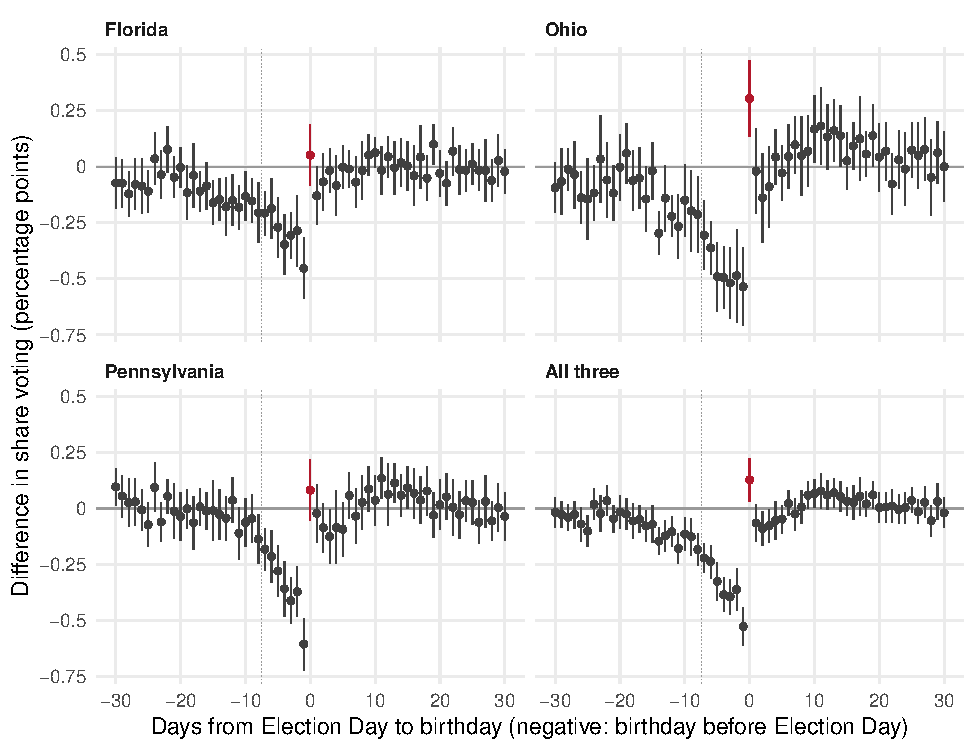
\includegraphics[width=\textwidth]{turnout.pdf}
\caption{Turnout by days between birthday and Election Day. Estimates relative to birthdays more than \window{} days from Election Day, with 95\% confidence intervals; the red point is a birthday on Election Day, and the dotted line marks the week before it.}
\label{fig:turnout}
\end{figure}

Table~\ref{tab:main} summarizes the daily estimates. For all three states together, a birthday the day before Election Day lowers turnout by \dayPooled{} points (SE \dayPooledSe{}), against a turnout of \dayPooledRate{} among people with such birthdays, a fall of about \dayPooledRelative{}. The estimates for the three states are close: \dayFl{} points in Florida, \dayOh{} in Ohio, and \dayPa{} in Pennsylvania. Averaged over the week before the birthday, the fall is \weekPooled{} points (SE \weekPooledSe{}); we chose the week after seeing Florida, and averaging over three days (\threeDaysPooled{}, SE \threeDaysPooledSe{}) or two weeks (\twoWeeksPooled{}, SE \twoWeeksPooledSe{}) tells the same story. An Election Day birthday, by contrast, raises turnout by \birthdayPooled{} points (SE \birthdayPooledSe{}), an estimate driven by Ohio (\birthdayOh{}); in Florida and Pennsylvania it is \birthdayFl{} and \birthdayPa{}.

\begin{table}[htbp]
\centering\TableStyle
\caption{Effects of a birthday near Election Day. Percentage points, with standard errors clustered by birth date in parentheses. Week before is the average over the seven days before the birthday.}
\label{tab:main}
\begin{adjustbox}{max width=\textwidth}
\begin{tabular}{llrrr}
\toprule
 & Outcome & Week before & Day before & Election Day \\
\midrule
Florida & Turnout & $-$0.29 (0.03) & $-$0.45 (0.07) & 0.05 (0.07) \\
 & In person on Election Day & $-$0.26 (0.03) & $-$0.65 (0.07) & $-$0.39 (0.07) \\
 & Early in person & $-$0.06 (0.02) & 0.16 (0.04) & 0.28 (0.05) \\
 & By mail & 0.03 (0.02) & 0.03 (0.04) & 0.16 (0.04) \\
Ohio & Turnout & $-$0.46 (0.06) & $-$0.54 (0.09) & 0.30 (0.09) \\
Pennsylvania & Turnout & $-$0.35 (0.04) & $-$0.61 (0.06) & 0.08 (0.07) \\
 & In person on Election Day & $-$0.40 (0.04) & $-$0.71 (0.06) & $-$0.11 (0.09) \\
 & By mail & 0.05 (0.02) & 0.10 (0.03) & 0.19 (0.05) \\
All three & Turnout & $-$0.35 (0.02) & $-$0.53 (0.04) & 0.13 (0.05) \\
\bottomrule
\end{tabular}

\end{adjustbox}
\end{table}

How people vote changes more than whether they vote (Figure~\ref{fig:methods}). In Florida and Pennsylvania the fall in turnout before a birthday is a fall in voting at the polls on Election Day: \pollsDayFl{} and \pollsDayPa{} points when the birthday is the day before. When the birthday falls a few days after Election Day, Floridians also vote at the polls less often, but voting early and by mail make up most of the difference, so turnout falls only slightly. A birthday reduces voting in person on other days as well: Floridians whose birthday falls in the last week of early voting, a week or so before Election Day, vote early less often. When Election Day is the birthday, Floridians are \pollsBirthdayFl{} points less likely to vote at the polls but \earlyBirthdayFl{} points more likely to vote early and \mailBirthdayFl{} points more likely to vote by mail, so turnout is unchanged. In Pennsylvania, which has no early in-person voting, voting by mail rises by \mailBirthdayPa{} points.

\begin{figure}[htbp]
\centering
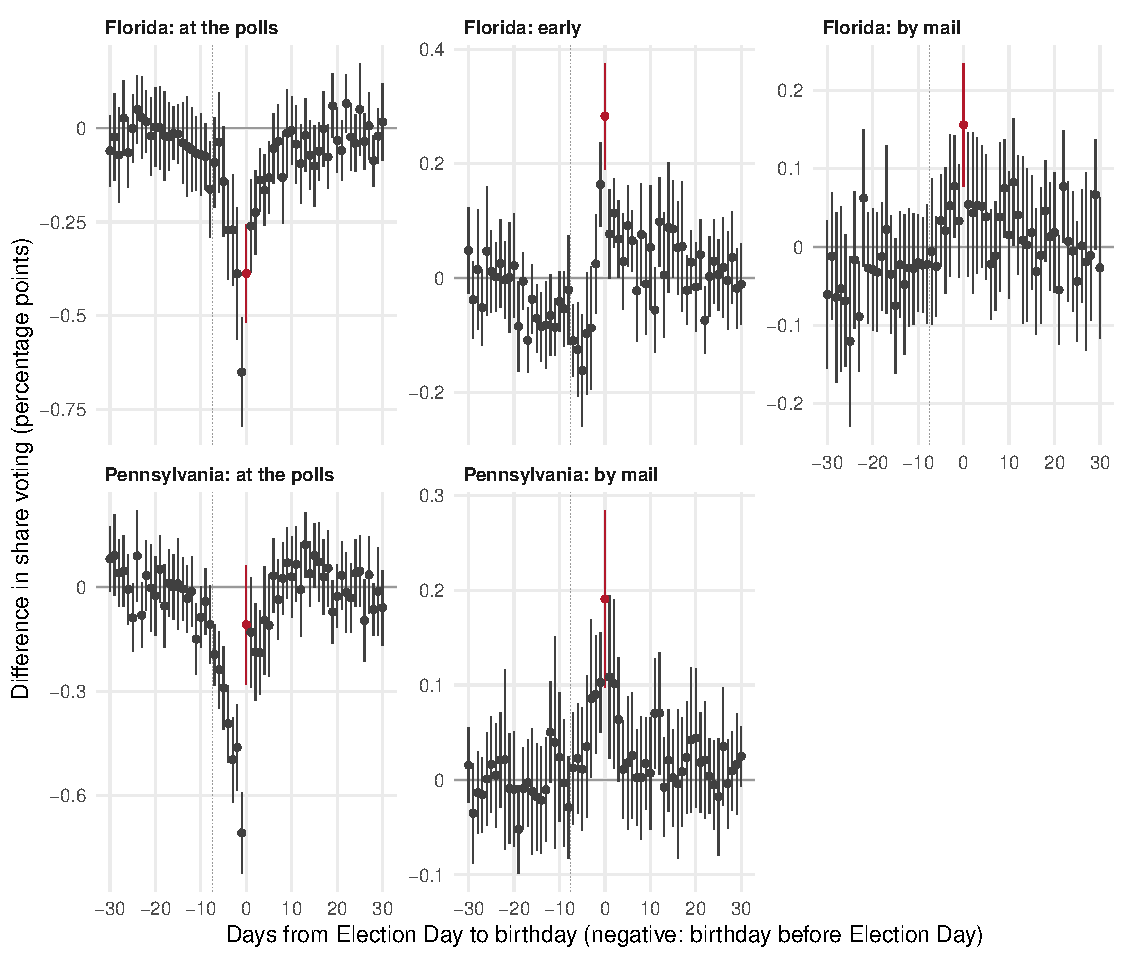
\includegraphics[width=\textwidth]{methods.pdf}
\caption{Voting by method and days between birthday and Election Day. Florida records voting at the polls, early, and by mail; Pennsylvania records voting at the polls and by mail or absentee ballot (shown together) and has no early in-person voting. Ohio does not record how people voted. Estimates and intervals as in Figure~\ref{fig:turnout}.}
\label{fig:methods}
\end{figure}

Table~\ref{tab:robustness} shows that the result does not depend on how standard errors are clustered; appears in general elections (\generalDay{} points the day before) and primaries (\primaryDay{}); and is as large in the samples that were not used to find it, \replicationDay{} points (SE \replicationDaySe{}) the day before, as in the one that was (\discoveryDay{}). Florida's 2018--2020 elections alone give \lateFlDay{} points (SE \lateFlDaySe{}). Nor is it the product of registration changes made at licence renewals. Among Ohio and Pennsylvania registrants whose latest registration came a year or more before the election, so that no registration change fell in the run-up to it, a birthday the day before lowers turnout by \settledDay{} points, against \allDay{} among all registrants in the two states.

\begin{table}[htbp]
\centering\TableStyle
\caption{Robustness of the turnout estimates for the three states together. Percentage points, standard errors in parentheses, clustered by birth date unless noted. $^a$The two-way clustered covariance matrix was not positive definite and was adjusted by setting negative eigenvalues to zero.}
\label{tab:robustness}
\begin{tabular}{lrrr}
\toprule
 & Week before & Day before & Election Day \\
\midrule
Main specification & $-$0.35 (0.02) & $-$0.53 (0.04) & 0.13 (0.05) \\
Clustered by birth date within state & $-$0.35 (0.02) & $-$0.53 (0.04) & 0.13 (0.05) \\
Clustered by birth date and by election$^a$ & $-$0.35 (0.03) & $-$0.53 (0.05) & 0.13 (0.05) \\
Florida 2006--2016 only & $-$0.33 (0.04) & $-$0.48 (0.08) & 0.06 (0.09) \\
All other elections & $-$0.38 (0.03) & $-$0.56 (0.05) & 0.17 (0.05) \\
\quad Florida 2018--2020 only & $-$0.33 (0.08) & $-$0.39 (0.17) & 0.17 (0.10) \\
General elections only & $-$0.64 (0.06) & $-$0.81 (0.08) & $-$0.04 (0.07) \\
Primaries only & $-$0.30 (0.03) & $-$0.45 (0.05) & 0.10 (0.07) \\
Ohio and Pennsylvania & $-$0.39 (0.03) & $-$0.58 (0.05) & 0.17 (0.06) \\
\quad registered a year or more before & $-$0.39 (0.03) & $-$0.58 (0.05) & 0.13 (0.06) \\
\bottomrule
\end{tabular}

\end{table}

\section{Interpretation}

The evidence does not fit the idea that people treat an Election Day birthday as an occasion to do their duty. Turnout rises little, if at all. In Florida, people with an Election Day birthday are less likely to vote at the polls, not more, and in Pennsylvania the estimate is also negative, though not distinguishable from zero. Nor does it show that a birthday off work makes voting easier.

It fits better the idea that a birthday competes with voting in person, and that whether it costs a vote depends on whether people see the clash coming. Voting in person falls on the days around a birthday, whether that day is Election Day or a day of early voting. When Election Day is the birthday, the clash is obvious, and people who would have voted at the polls vote early or by mail instead, so turnout holds up. When the birthday falls a few days before Election Day, the clash is less obvious. The celebration, the trip, or the day off comes first, Election Day arrives while it is still going on or just after, and some of those who would have voted in person do not vote at all.

The data cannot say what people do on and around their birthdays, so this account is an interpretation rather than a finding. Three features of the evidence support it: the loss is in voting in person and not by mail; it is concentrated in the days just before Election Day rather than spread over the month; and voting early or by mail rises when the birthday is Election Day. Its leading mechanical alternative, registration changes made at driver's licence renewals, does not account for the pattern. The asymmetry is also hard to square with explanations that do not involve the birthday as an event, such as seasonality, which the design absorbs.

The effects are small. A fall of half a percentage point among the roughly one in 365 registrants whose birthday is the day before an election changes no election. But they show that turnout responds to modest, predictable demands on a person's time in the days around an election, and that the option to vote on another day absorbs some of that cost when people anticipate it.

\bibliographystyle{apsr}
\bibliography{references}

\clearpage
\appendix
\section{Turnout by Election}

\begingroup\small
\begin{longtable}{llrrrr}
\caption{Registrants and turnout by election. Turnout is the share of registrants in the analysis sample who voted; Official is the state's reported turnout where we could verify it.}\label{tab:elections}\\
\toprule
State & Election & Registrants & Turnout & Official & Birthday on E-Day \\
\midrule
\endfirsthead
\toprule
State & Election & Registrants & Turnout & Official & Birthday on E-Day \\
\midrule
\endhead
\bottomrule
\endlastfoot
Florida & Sep 5, 2006 PRI & 7,275,221 & 21.0\% & 20\% & 20,771 \\
 & Nov 7, 2006 GEN & 7,346,234 & 50.7\% & 47\% & 20,500 \\
 & Jan 29, 2008 PPP & 7,804,524 & 43.8\% & 42\% & 20,494 \\
 & Aug 26, 2008 PRI & 8,213,432 & 18.2\% & 18\% & 23,695 \\
 & Nov 4, 2008 GEN & 8,575,718 & 80.1\% & 75\% & 24,136 \\
 & Aug 24, 2010 PRI & 9,216,016 & 22.6\% & 22\% & 26,430 \\
 & Nov 2, 2010 GEN & 9,299,145 & 50.9\% & 49\% & 25,845 \\
 & Jan 31, 2012 PPP & 9,790,560 & 16.5\% & 41\% & 25,652 \\
 & Aug 14, 2012 PRI & 10,189,899 & 20.7\% & 21\% & 29,246 \\
 & Nov 6, 2012 GEN & 10,507,462 & 73.7\% & 72\% & 28,934 \\
 & Aug 26, 2014 PRI & 11,503,073 & 17.0\% & 18\% & 33,069 \\
 & Nov 4, 2014 GEN & 11,616,728 & 49.5\% & 51\% & 32,529 \\
 & Mar 15, 2016 PPP & 12,519,303 & 32.5\% & 46\% & 34,295 \\
 & Aug 30, 2016 PRI & 12,894,121 & 22.5\% & 24\% & 36,991 \\
 & Nov 8, 2016 GEN & 13,174,364 & 70.8\% & 75\% & 36,841 \\
 & Aug 28, 2018 PRI & 12,082,114 & 26.9\% & 27\% & 35,121 \\
 & Nov 6, 2018 GEN & 12,267,419 & 62.3\% & 63\% & 34,073 \\
 & Mar 17, 2020 PPP & 13,381,904 & 21.3\% & 30\% & 35,946 \\
 & Aug 18, 2020 PRI & 13,677,239 & 27.1\% & 28\% & 39,482 \\
 & Nov 3, 2020 GEN & 14,131,109 & 75.5\% & 77\% & 39,551 \\
Ohio & Mar 7, 2000 PRI & 2,437,416 & 47.6\% & -- & 6,585 \\
 & Nov 7, 2000 GEN & 2,841,507 & 86.3\% & -- & 7,731 \\
 & Nov 6, 2001 GEN & 3,464,860 & 47.7\% & -- & 9,393 \\
 & May 7, 2002 PRI & 3,550,654 & 24.6\% & -- & 9,299 \\
 & Nov 5, 2002 GEN & 3,608,309 & 60.7\% & -- & 9,814 \\
 & Nov 4, 2003 GEN & 3,757,964 & 43.5\% & -- & 10,328 \\
 & Mar 2, 2004 PRI & 3,841,226 & 41.4\% & -- & 10,365 \\
 & Nov 2, 2004 GEN & 4,077,784 & 90.9\% & -- & 11,112 \\
 & Nov 8, 2005 GEN & 4,693,490 & 50.4\% & -- & 12,705 \\
 & May 2, 2006 PRI & 4,763,348 & 30.0\% & -- & 12,520 \\
 & Nov 7, 2006 GEN & 4,820,526 & 67.4\% & -- & 13,064 \\
 & Nov 6, 2007 GEN & 4,978,821 & 34.9\% & -- & 13,471 \\
 & Mar 4, 2008 PRI & 5,057,829 & 57.4\% & -- & 13,818 \\
 & Nov 4, 2008 GEN & 5,284,519 & 86.2\% & 69.97\% & 14,450 \\
 & Nov 3, 2009 GEN & 5,674,587 & 50.0\% & -- & 15,400 \\
 & May 4, 2010 PRI & 5,766,412 & 27.2\% & -- & 15,038 \\
 & Nov 2, 2010 GEN & 5,829,994 & 59.6\% & -- & 15,768 \\
 & Nov 8, 2011 GEN & 6,017,965 & 54.5\% & -- & 16,281 \\
 & Mar 6, 2012 PRI & 6,124,785 & 29.2\% & -- & 16,495 \\
 & Nov 6, 2012 GEN & 6,312,807 & 79.8\% & 70.53\% & 17,115 \\
 & Nov 5, 2013 GEN & 6,684,151 & 29.2\% & -- & 18,103 \\
 & May 6, 2014 PRI & 6,787,236 & 18.2\% & -- & 17,807 \\
 & Nov 4, 2014 GEN & 6,873,345 & 43.7\% & -- & 18,578 \\
 & Nov 3, 2015 GEN & 7,125,003 & 44.2\% & -- & 19,261 \\
 & Mar 15, 2016 PRI & 7,269,254 & 44.3\% & -- & 20,137 \\
 & Nov 8, 2016 GEN & 7,598,098 & 71.8\% & 71.33\% & 20,703 \\
Pennsylvania & Nov 3, 2009 GEN & 5,089,456 & 24.6\% & -- & 13,712 \\
 & May 18, 2010 PRI & 5,140,352 & 24.5\% & -- & 13,955 \\
 & Nov 2, 2010 GEN & 5,183,081 & 50.9\% & -- & 13,972 \\
 & May 17, 2011 PRI & 5,259,914 & 20.6\% & -- & 14,033 \\
 & Nov 8, 2011 GEN & 5,305,951 & 27.0\% & -- & 14,452 \\
 & Apr 24, 2012 PRI & 5,378,732 & 20.2\% & -- & 14,182 \\
 & Nov 6, 2012 GEN & 5,503,735 & 70.3\% & 67.63\% & 15,013 \\
 & May 21, 2013 PRI & 5,684,730 & 15.3\% & -- & 15,096 \\
 & Nov 5, 2013 GEN & 5,729,058 & 22.9\% & -- & 15,780 \\
 & May 20, 2014 PRI & 5,791,363 & 17.1\% & -- & 15,431 \\
 & Nov 4, 2014 GEN & 5,843,440 & 45.3\% & -- & 15,720 \\
 & May 19, 2015 PRI & 5,929,854 & 20.0\% & -- & 15,812 \\
 & Nov 3, 2015 GEN & 6,000,477 & 29.4\% & -- & 16,088 \\
 & Apr 26, 2016 PRI & 6,157,174 & 42.9\% & -- & 16,200 \\
 & Nov 8, 2016 GEN & 6,437,720 & 73.8\% & 70.11\% & 17,524 \\
 & May 16, 2017 PRI & 6,723,220 & 17.7\% & -- & 18,151 \\
 & Nov 7, 2017 GEN & 6,772,403 & 27.3\% & -- & 18,422 \\
 & May 15, 2018 PRI & 6,858,484 & 19.7\% & -- & 18,563 \\
 & Nov 6, 2018 GEN & 6,959,206 & 60.6\% & -- & 18,979 \\
 & May 21, 2019 PRI & 7,157,787 & 20.6\% & -- & 19,186 \\
 & Nov 5, 2019 GEN & 7,244,125 & 33.6\% & -- & 19,913 \\
 & Jun 2, 2020 PRI & 7,454,732 & 33.5\% & -- & 20,372 \\
 & Nov 3, 2020 GEN & 7,836,509 & 76.6\% & 76.07\% & 21,111 \\
 & May 18, 2021 PRI & 8,017,039 & 27.2\% & -- & 21,795 \\
 & Nov 2, 2021 GEN & 8,074,129 & 32.7\% & -- & 21,652 \\
 & May 17, 2022 PRI & 8,167,450 & 31.1\% & -- & 22,026 \\
 & Nov 8, 2022 GEN & 8,306,757 & 61.4\% & -- & 22,516 \\
 & May 16, 2023 PRI & 8,438,870 & 24.2\% & -- & 22,795 \\
 & Nov 7, 2023 GEN & 8,519,314 & 36.5\% & -- & 23,052 \\
 & Apr 23, 2024 PRI & 8,659,086 & 24.1\% & -- & 22,757 \\
\end{longtable}

\endgroup

\end{document}
